\section{Решающие деревья}

\textbf{Дерево принятия решений}  — средство поддержки принятия решений.

Структура дерева представляет собой «листья» и «ветки». На рёбрах («ветках») дерева решения записаны признаки, от которых зависит целевая функция, в «листьях» записаны значения целевой функции, а в остальных узлах — признаки, по которым различаются случаи.

Чтобы классифицировать новый случай, надо спуститься по дереву до листа и выдать соответствующее значение.

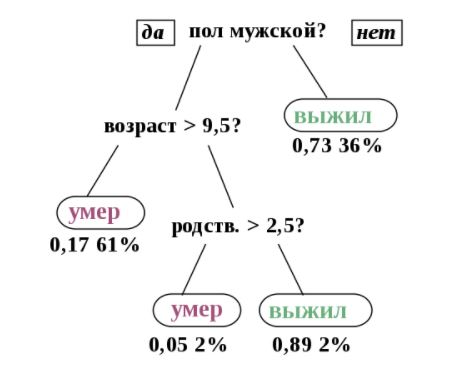
\includegraphics[]{tickets/pictures/1.JPG}

\subsection{Энтропия}


\subsubsection{Энтропия состояния системы}
$$
S=-\sum_{i=1}^{N} p_{i} \log _{2} p_{i}
$$
где $\mathrm{p}_{i} $ --- вероятности нахождения системы в і-ом состоянии.
Интуитивно, энтропия соответствует степени хаоса в системе.
Чем выше \textit{энтропия}, тем менее упорядочена система и наоборот.

\subsubsection{Прирост информации}

Поскольку \textit{энтропия} - по сути степень хаоса в системе, уменьшение \textit{энтропии} называют \textbf{приростом информации}. Формально \textit{прирост информации} (\textit{information gain, IG}) при разбиении выборки по признаку Q (например признаком Q может быть « $\mathrm{x} \leq 12$ ») определяется как
$$
I G(Q)=S_{O}-\sum_{i=1}^{q} \frac{N_{i}}{N} S_{i}
$$


где $q$ --- число групп после разбиения, $N_i$ --- число элементов выборки, у которых признак $Q$ имеет $і$-ое значение.

\subsection{Алгоритм построения решающего дерева.}

Интуитивно на каждом шаге мы хотим задавать вопрос, который давал бы максимальное количество информации и лучше всего бы на конкретном шаге разделял выборку.

В алгоритмах используется \textbf{принцип жадной максимизации прироста информации} --- на каждом шаге выбирается тот признак, при разделении по которому \textit{прирост информации} оказывается \textit{наибольшим}.

Дальше процедура повторяется рекурсивно, пока энтропия не окажется равной нулю или какой-то малой величине.
В разных алгоритмах применяются разные эвристики для "ранней остановки" или "отсечения", чтобы избежать построения переобученного дерева.


\subsubsection{Критерии останова при построения дерева}

\begin{itemize}
    \item  Ограничение максимальной глубины дерева.
    \item  Ограничение минимального числа объектов в листе.
    \item  Ограничение максимального количества листьев в дереве.
    \item  Остановка в случае, если все объекты в листе относятся к одному классу.
    \item  Требование, что функционал качества при дроблении улучшался как минимум на х процентов.
\end{itemize}
\subsection{Кросс-энтропия.}

\textbf{Кросс-энтропия} --- мера разности между распределениями (Вроде тут вместо кросс-энтропии должна быть просто энтропия).


